\documentclass[tikz,border=1pt]{standalone}
\usepackage{fancyvrb}
\usepackage{pgf}
\usepackage{tikz}
\usetikzlibrary{arrows,automata,positioning}
\usepackage[latin1]{inputenc}

\begin{document}
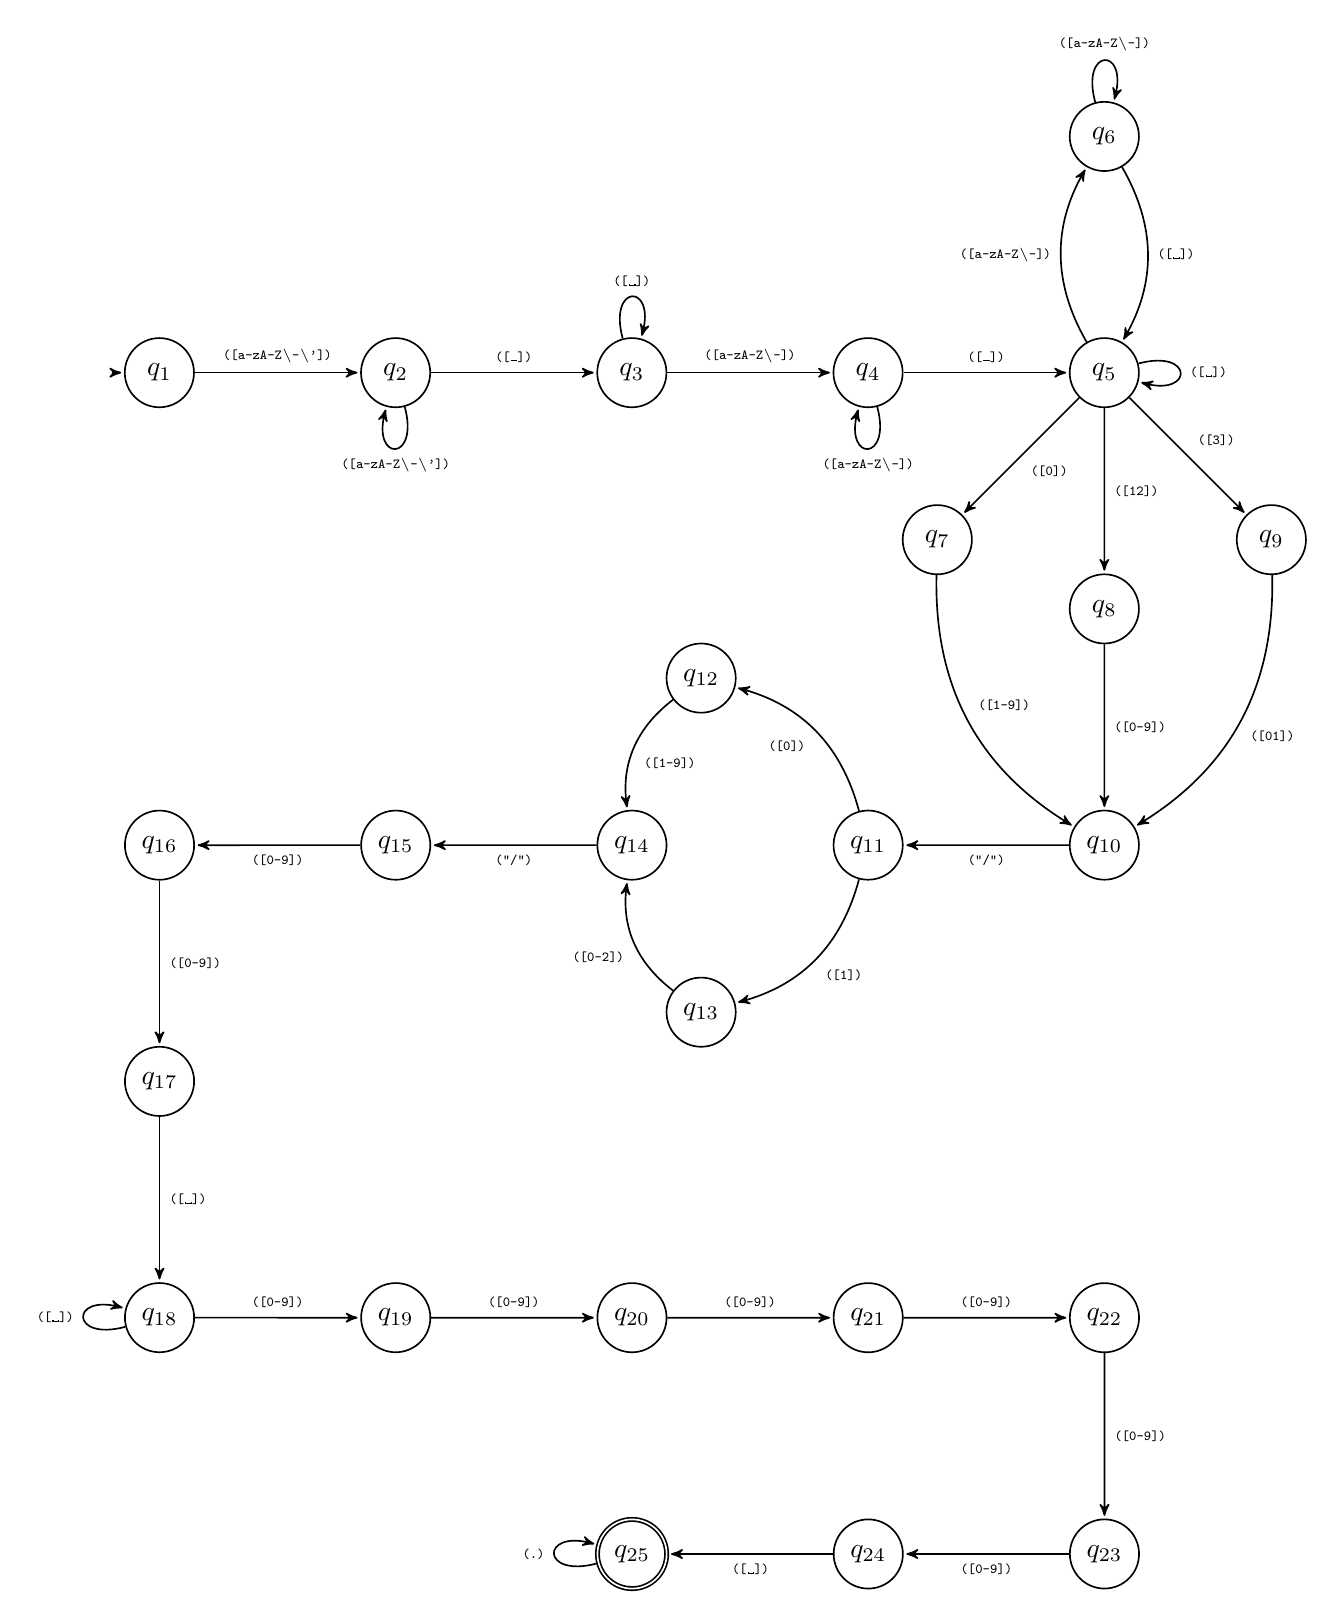
\begin{tikzpicture}[->,>=stealth',shorten >=1pt,auto,node distance=3cm,on grid,semithick,initial text=,scale=0.3]
%\tikzstyle{every state}=[fill=none,text=yellow]
\tikzset{every edge/.append style={font=\tiny}}

\node[initial,state] 	(1)			{$q_1$};
\node[state]         	(2)	[right of=1]	{$q_2$};
\node[state]		(3)	[right of=2]	{$q_3$};
\node[state]		(4)	[right of=3]	{$q_4$};
\node[state]		(5)	[right =of 4]	{$q_5$};
\node[state]		(6)	[above of=5]	{$q_6$};
\node[state]		(7)	[below left of=5]	{$q_7$};
\node[state]		(8)	[below of=5]	{$q_8$};
\node[state]		(9)	[below right of=5]	{$q_9$};
\node[state]		(10)	[below of=8]	{$q_{10}$};
\node[state]		(11)	[left =of 10]	{$q_{11}$};
\node[state]		(12)	[above left of=11]	{$q_{12}$};
\node[state]		(13)	[below left of=11]	{$q_{13}$};
\node[state]		(14)	[left of=11]	{$q_{14}$};
\node[state]		(15)	[left  of=14]	{$q_{15}$};
\node[state]		(16)	[left of=15]	{$q_{16}$};
\node[state]		(17)	[below of=16]	{$q_{17}$};
\node[state]		(18)	[below of=17]	{$q_{18}$};
\node[state]		(19)	[right of=18]	{$q_{19}$};
\node[state]		(20)	[right of=19]	{$q_{20}$};
\node[state]		(21)	[right of=20]	{$q_{21}$};
\node[state]		(22)	[right  of=21]	{$q_{22}$};
\node[state]		(23)	[below of=22]	{$q_{23}$};
\node[state]		(24)	[left of=23]	{$q_{24}$};
\node[state,accepting]  (25)	[left of=24]	{$q_{25}$};
                                          
\path	(1)	edge			node	{\texttt{([a-zA-Z\textbackslash\\-\textbackslash\\'])}}	(2)

	(2)	edge			node	{\texttt{([\textvisiblespace])}}	(3)
		edge	[loop below]	node	{\texttt{([a-zA-Z\textbackslash\\-\textbackslash\\'])}}	(2)
      	

	(3)	edge			node	{\texttt{([a-zA-Z\textbackslash\\-])}}	(4)
		edge	[loop above]	node	{\texttt{([\textvisiblespace])}}	(3)

	(4)	edge			node	{\texttt{([\textvisiblespace])}}	(5)
		edge	[loop below]	node	{\texttt{([a-zA-Z\textbackslash\\-])}}	(4)

	(5)	edge	[bend left]	node	{\texttt{([a-zA-Z\textbackslash\\-])}}	(6)
		edge			node	{\texttt{([0])}}	(7)
		edge			node	{\texttt{([12])}}	(8)
		edge			node	{\texttt{([3])}}	(9)
		edge	[loop right]	node	{\texttt{([\textvisiblespace])}}	(9)

	(6)	edge	[bend left]	node	{\texttt{([\textvisiblespace])}}	(5)
		edge	[loop above]	node	{\texttt{([a-zA-Z\textbackslash\\-])}}	(6)

	(7)	edge	[bend right]	node	{\texttt{([1-9])}}	(10)
	(8)	edge			node	{\texttt{([0-9])}}	(10)
	(9)	edge	[bend left]	node	{\texttt{([01])}}	(10)
	(10)	edge			node	{\texttt{("/")}}	(11)

	(11)	edge	[bend right]	node	{\texttt{([0])}}	(12)
		edge	[bend left]	node	{\texttt{([1])}}	(13)

	(12)	edge	[bend right]	node	{\texttt{([1-9])}}	(14)
	(13)	edge	[bend left]	node	{\texttt{([0-2])}}	(14)
	(14)	edge			node	{\texttt{("/")}}	(15)
	(15)    edge			node	{\texttt{([0-9])}}	(16)
	(16)    edge			node	{\texttt{([0-9])}}	(17)
	(17)    edge			node	{\texttt{([\textvisiblespace])}}	(18)

        (18)    edge			node	{\texttt{([0-9])}}	(19)
		edge	[loop left]	node	{\texttt{([\textvisiblespace])}}	(18)

        (19)    edge			node	{\texttt{([0-9])}}	(20)
        (20)    edge			node	{\texttt{([0-9])}}	(21)
        (21)    edge			node	{\texttt{([0-9])}}	(22)
        (22)	edge			node	{\texttt{([0-9])}}	(23)
        (23)	edge			node	{\texttt{([0-9])}}	(24)
        (24)	edge			node	{\texttt{([\textvisiblespace])}}	(25)
	(25)	edge	[loop left]	node	{\texttt{(.)}}	(25);
\end{tikzpicture}
\end{document}
%
%COGNOME	([a-zA-Z\-\']+)
%NOME		(([a-zA-Z\-])+([ ]+[a-zA-Z\-]+)*)
%
%GIORNO		((0?[1-9])|([12][0-9])|3[01])
%MESE		((0?[1-9])|(1[0-2]))
%ANNO		((0?[0-9])|([1-9][0-9]))
%
%SEP		("/")
%MATRICOLA	([0-9]+{6})
%WHITESPACE	([\textvisiblespace]+)
%COMMENTI	(.*)
%
